\chapter{Rule Retrieval with HFiles}
\label{chap:hfile}

% TODO check for duplicates in bibliography

Data availability and distributed computing techniques have allowed SMT
researchers to build larger translation models. However, decoders need to be
able to retrieve information efficiently from these models to be able to
translate an input sentence or a set of input sentences. We introduce an easy to
implement and general purpose solution to tackle this problem: we store
translation models as a set of key-value pairs in an HFile. We apply this
strategy to test set hierarchical phrase-based rule filtering. We compare our
approach to alternative strategies and show that its trade offs in terms
of speed, memory and simplicity are
competitive~\citep{pino-waite-byrne:2012:PBML}. Software written for this work
is available at \url{https://github.com/jmp84/ruleXtract} (branch PBML-2012).

\section{Introduction}

Current machine translation research is characterised by increasing amounts
of available data. For example, \autoref{fig:wmtdata} shows that
for the WMT machine translation
workshop~\citep{bojar-buck-callisonburch-federmann-haddow-koehn-monz-post-soricut-specia:2013:WMT}
French-English constrained track translation task, the English side of parallel
data has increased from 13.8M tokens in 2006 to 1012.7M tokens in 2012 and that
available English monolingual data has increased from 27.5M tokens to 6852.7M
tokens.
%
\begin{figure}
  \begin{center}
    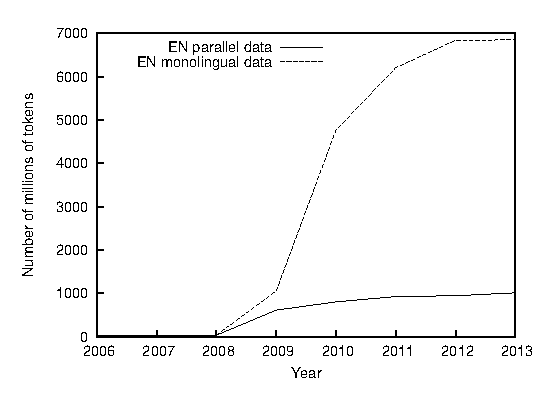
\includegraphics[scale=0.8]{figures/wmt/wmtdata.eps}
    \caption{Number of English tokens (in millions) in parallel and monolingual
      data available for the WMT translation shared task constrained track for
      the years 2006 to 2013.}
    \label{fig:wmtdata}
  \end{center}
\end{figure}
%
Along with growing amounts of data, the use of more powerful computers
and distributed computing models such as
MapReduce~\citep{dean-ghemawat:2008:ACM,lin-dyer:2010:book} has enabled machine
translation researchers to build larger statistical machine translation models.
Examples include language
modelling~\citep{brants-popat-xu-och-dean:2007:EMNLP-CoNLL}, translation rule
extraction~\citep{dyer-cordova-mont-lin:2008:WMT,weese-ganitkevitch-callisonburch-post-lopez:2011:WMT},
word alignment~\citep{dyer-cordova-mont-lin:2008:WMT,lin-dyer:2010:book} as well
as end-to-end toolkits for building entire
phrase-based~\citep{gao-vogel:2010:PBML} or hierarchical phrase-based
models~\citep{venugopal-zollmann:2009:PBML} using MapReduce.

Once SMT models are built, decoders only need a fraction of the information
contained in those models to be able to translate an input source sentence or a
set of input source sentences. For example, in translation from French to
English, given an input sentence \emph{Salut toi}, we only need to know the
translation probabilities the model assigns to the words \emph{Salut} and
\emph{toi} and to the phrase \emph{Salut toi}.
With larger models, simply retrieving relevant translation
probabilities becomes a challenge. Given a test set, the decoder
only needs the rules whose source side matches part of one of the source
sentences in the test set to be able to generate hypotheses. In the system
described by \citet{iglesias-degispert-banga-byrne:2009:NAACL}, for each
new test set, rules are re-extracted and filtered at extraction time. This
method becomes progressively slower with larger amounts of data and we
would like to improve on it for more rapid experimentation. We also would like
to use as lightweight a computing infrastructure as possible. For example, HBase
has been applied to the use of distributed language
models~\citep{yu:2008:mastersthesis}. However, we wish to address the question
whether we can adapt this heavy infrastructure to our purposes with minimal
effort. Rule filtering is an essential step in our pipeline that can be a
bottleneck. Our goal is to reduce its processing time from several hours to a
few minutes.

In this chapter, we address the problem of retrieving relevant translation
model probabilities by storing the model in the HFile data
structure.\footnote{\url{http://hbase.apache.org}} To our knowledge, this is the first
detailed proposed implementation of translation model storage and
filtering using HFile data structures. We believe it offers a good compromise
between speed, performance and ease of implementation. Although the HFile
construction is done via MapReduce and a cluster of machines, the infrastructure
for filtering is lightweight and requires the use of only one machine. We will
apply this approach to test set rule filtering prior
to decoding. We will discuss alternative
strategies as well as their strengths and weaknesses in terms of speed and
memory usage. In \autoref{sec:relatedwork}, we will review approaches that
have been used for model filtering. The HFile data structure that is used to
store models will be presented in \autoref{sec:hfile}. Our method and
alternative strategies will be compared empirically in
\autoref{sec:rulextract}. We will finally conclude in \autoref{sec:conclusion}.

\section{Related Work}
\label{sec:relatedwork}

We now review techniques appearing in the literature that have been used to
store SMT models and to retrieve the information needed in translation from
these models. SMT models are usually discrete probabilistic models and can
therefore be represented as a set of key-value pairs. To obtain relevant
information from a model stored in a data structure, a set of keys called a
\emph{query set} is formed, then each key in this query set is looked up in the
model. Strategies include storing the model as a simple data structure in
memory, in a plain text file, in more complicated data structures in memory,
storing fractions of the entire model, simply storing data as opposed to a
precomputed model or storing models in a distributed fashion.

If small enough, it may be possible to fit the model into physical memory. In
this case the model can be stored as a memory associative array, such as a hash
table, for rapid query retrieval. In-memory storage has been used to store model
parameters between iterations of expectation-maximisation for word
alignment~\citep{dyer-cordova-mont-lin:2008:WMT,lin-dyer:2010:book}.

For larger models, the set of key-value pairs can be stored as a table in a
single text file on local disk. Values for keys in the query set are retrieved
by scanning through the entire file. For each key in the file, its membership is
tested in the query set. This is the approach adopted in the \emph{Joshua 5.0}
decoder~\citep{post-ganitkevitch-orland-weese-cao-callisonburch:2013:WMT}\footnote{The
publication does not mention this, we simply infer it from the decoder training
scripts available at \url{http://joshua-decoder.org/5.0/index.html}.}, which
uses regular expressions or $n$-grams to test membership.
\citet{venugopal-zollmann:2009:PBML} use MapReduce to scan a file concurrently:
a mapper is defined that tests if the vocabulary of a rule matches the
vocabulary of a test set. The MapReduce framework then splits the grammar file
into subsections for the mappers to scan over in parallel.

The model can also be stored using a trie associative
array~\citep{fredkin:1960:ACM}. A trie is a type of tree where each node
represents a shared prefix of a set of keys represented by the child nodes. Each
node only stores the prefix it represents. The keys are therefore compactly
encoded in the structure of the trie itself. Querying the trie is a
$\mathcal{O}(\log(n))$ operation, where $n$ is the number of keys in the
dataset. The trie may also be small enough to fit in physical memory to further
reduce querying time. Tries have been used for storing phrase
tables~\citep{zens-ney:2007:HLTNAACL}, hierarchical phrase-based
grammars~\citep{ganitkevitch-cao-weese-post-callisonburch:2012:WMT} and
language models~\citep{pauls-klein:2011:HLTACL,heafield:2011:WMT}.

It is also possible to create a much smaller approximate version of the model.
Randomised language
models~\citep{talbot-osborne:2007:ACL,talbot-osborne:2007:EMNLP-CoNLL,talbot-brants:2008:ACL}
store parameters or counts associated with $n$-grams in a structure similar to a
Bloom filter~\citep{bloom:1970:ACM}. This structure is small in comparison to
the original language model, although the reduction in size comes at the cost of
randomly corrupting model parameters or assigning model parameters to unseen
$n$-grams. \citet{guthrie-hepple:2010:EMNLP} propose an extension which prevents
the random corruption of model parameters but does not stop the random
assignment of parameters to unseen $n$-grams.
\citet{levenberg-osborne:2009:EMNLP} extend randomised language models to
stream-based language models. Another way of building a smaller approximate
version of a model is to retain items with high frequency counts from a stream
of data~\citep{manku-motwani:2002:VLDB}. This technique has been applied to
language modelling~\citep{goyal-daumeiii-venkatasubramanian:2009:NAACL} and
translation rule extraction~\citep{przywara-bojar:2011:PBML}. 

Instead of pre-computing the dataset it is possible to compute the sufficient
statistics at query time using a suffix array~\citep{manber-myers:1990:SIAM}, so
that the model can be estimated on the fly. A suffix array is a sequence of
pointers to each suffix in a training corpus. The sequence is sorted with
respect to the lexicographic order of the referenced suffixes. Suffix arrays
have been used for computing statistics for language
models~\citep{zhang-vogel:2006:techreport}, phrase-based
systems~\citep{callisonburch-bannard-schroeder:2005:ACL,zhang-vogel:2005:EAMT},
and hierarchical phrase-based systems~\citep{lopez:2007:EMNLP-CoNLL}.

Finally, some approaches store language models in a distributed fashion.
\citet{brants-popat-xu-och-dean:2007:EMNLP-CoNLL} describe a distributed, fast,
low-latency infrastructure for storing very large language models.
\citet{zhang-hildebrand-vogel:2006:EMNLP} propose a distributed large language
model backed by suffix arrays. HBase has also been used to build a distributed
language infrastructure~\citep{yu:2008:mastersthesis}. The method we propose to
use is closely related to the latter but we use a more lightweight
infrastructure than HBase. In addition, it is also possible to apply the method
to language model querying~\citep{pino-waite-byrne:2012:PBML}, which
demonstrates the flexibility of the infrastructure.

\section{HFile Description}
\label{sec:hfile}

We now describe the data structure we use to store models and we review relevant
features to the design of our system. To store a model represented as key-value
pairs, we use the HFile file format,\footnote{\url{http://hbase.apache.org}} which is
a reimplementation of the SSTable file
format~\citep{chang-dean-ghemawat-hsieh-wallach-burrows-chandra-fikes-gruber:2008:ACM}.
The HFile is used at a lower level in the HBase infrastructure. In this work, we
reuse the HFile format directly without having to install an HBase system. The
HFile format is a lookup table with key and value columns. The entries are free
to be an arbitrary string of bytes of any length. The table is sorted
lexicographically by the key byte string for efficient record retrieval by key.

\subsection{Internal structure}

As can be seen in \autoref{fig:hfile}, the data contained in an HFile is
internally organised into blocks called data blocks. The block size is
configurable, with a default size of 64KB. Note that HFile blocks are not to be
confused with Hadoop Distributed File System (HDFS) blocks whose default size is
64MB. If an HFile is stored on HDFS, several HFile blocks will be contained in
an HDFS block. A block index is constructed which maps the first key of an HFile
block to the location of the block in the file. For large HFiles the block index
can be very large. Therefore the block index is itself organised into blocks,
which are called leaf index blocks. These leaf index blocks are interspersed
with the data blocks in the HFile. In turn, the leaf index blocks are indexed by
intermediate level data index blocks. The intermediate blocks are then indexed
by a root data index. The root data index and optionally the Bloom filter
metadata, described next, are stored at the end of the HFile. In order to
distinguish block types (data block, index block, etc.), the first 8 bytes of a
block will indicate the type of block being read. The HFile format allows for
the blocks to be compressed. The choice of compression codec is selected when
the file is created. We choose the GZip compression codec for all our
experiments. Block compression is also used in other related
software~\citep{pauls-klein:2011:HLTACL}. For more details, the interested
reader can refer to the HBase
documentation.\footnote{\url{http://hbase.apache.org/book/book.html}}

\begin{figure}
  \begin{center}
    \begin{tabular}{|l|}
      \hline
      \rowcolor[gray]{0.85}
      Data Block \\
      \hline
      \rowcolor[gray]{0.86}
      ... \\
      \hline
      \rowcolor[gray]{0.95}
      Leaf index block / Bloom block \\
      \hline
      \rowcolor[gray]{0.86}
      ... \\
      \hline
      \rowcolor[gray]{0.85}
      Data Block \\
      \hline
      \rowcolor[gray]{0.86}
      ... \\
      \hline
      \rowcolor[gray]{0.95}
      Leaf index block / Bloom block \\
      \hline
      \rowcolor[gray]{0.86}
      ... \\
      \hline
      \rowcolor[gray]{0.85}
      Data Block \\
      \hline
      \rowcolor[gray]{0.7}
      Intermediate Level Data Index Blocks \\
      \hline
      \rowcolor[gray]{0.6}
      Root Data Index \\
      \hline
      \rowcolor[gray]{0.6}
      File Info \\
      \hline
      \rowcolor[gray]{0.6}
      Bloom Filter Metadata \\
      \hline
    \end{tabular}
    \caption[Caption for LOF]{HFile internal structure.\footnotemark}
    \label{fig:hfile}
  \end{center}
\end{figure}

\footnotetext{after \url{http://hbase.apache.org/book/book.html} (simplified)}

\subsection{Record retrieval}

When the HFile is opened for reading, the root data index is loaded into memory.
To retrieve a value from the HFile given a key, the appropriate intermediate
index block is located by a binary search through the root data index. Binary
searches are conducted on the intermediate and leaf index blocks to identify the
data block that contains the key. The data block is then loaded off the disk
into memory and the key-value record is retrieved by scanning the data block
sequentially.

\subsection{Bloom filter optimization}

It is possible to query for a key that is not contained in the HFile. This very
frequently happens in translation because of language data sparsity. Querying
the existence of a key is expensive as three blocks have to be loaded from disk
and binary searched. For fast existence check queries, the HFile format allows
the inclusion of an optional Bloom filter~\citep{bloom:1970:ACM}. A Bloom filter
provides a probabilistic, memory efficient representation of the key set with a
$\mathcal{O}(1)$ membership test operation. The Bloom filter may provide a false
positive,
but never a false negative for existence of a key in the HFile. For a large
HFile, the Bloom filter may also be very large. Therefore the  Bloom filter is
also organised into blocks called Bloom blocks. Each block contains a smaller
Bloom filter that covers a range of keys in the HFile. Similar to the root data
index, a Bloom filter metadata or Bloom index is constructed. To check for the
existence of a key, a binary search is conducted on the Bloom index, the
relevant Bloom block is loaded, and the membership test performed. Contrary to
work on Bloom filter language
model~\citep{talbot-osborne:2007:ACL,talbot-osborne:2007:EMNLP-CoNLL}, this
filter only tests the existence of a key and does not return any statistics from
the value. If a membership test is positive, the HFile data structure still
requires to do a usual search. During the execution of a query, two keys may
reference the same index or Bloom blocks. To prevent these blocks from being
repeatedly loaded from disk, the blocks are cached after reading.

\subsection{Local disk optimization}

The HFile format is designed to be used with HDFS, a distributed file system
based on the Google File System~\citep{ghemawat-gobioff-leung:2003:OSP}. Large
files are split into HDFS blocks that are stored on many nodes in a cluster.
However, the HFile format can also be used completely independently of HDFS. If
its size is smaller than disk space, the entire HFile can be stored on the local
disk of one machine and accessed through the machine's local file system. We
find in \autoref{sec:rulextract} that using local disk
is faster than using HDFS.

\subsection{Query sorting optimization}

Prior to HFile lookup, we sort keys in the query set lexicographically. If two
keys in the set of queries are contained in the same block, then the block is
only loaded once. In addition, the computer hardware and operating system allow
further automatic improvements to the query execution. Examples of these
automatic improvements include reduced disk seek time, the operating system
caching data from
disk,\footnote{The Linux Documentation Project, The File System, \url{http://tldp.org}}
or CPU caching data from main memory~\citep{patterson-hennessy:2005:COA}.

\section{Hierarchical Rule Extraction with MapReduce}
\label{sec:rulextractMapReduce}

In this section, we describe a MapReduce implementation of hierarchical rule
extraction. The implementation is based on Method 3 described by
\citet{dyer-cordova-mont-lin:2008:WMT}.
MapReduce~\citep{dean-ghemawat:2008:ACM} is a framework designed for processing
large amounts of data in a distributed fashion on a computer cluster. In this
framework, the programmer needs to implement a function called \emph{map} and
a function called \emph{reduce}. The \emph{map} function is defined in
\autoref{eq:mapFunction}.
%
\begin{equation}
  \text{map} : (k_1, v_1) \longmapsto [(k_2, v_2)]
  \label{eq:mapFunction}
\end{equation}
%
$(k_1, v_1)$ is a key-value pair and $[(k_2, v_2)]$ is a list of
key-value pairs. Keys and values are arbitrary byte sequences. Behind the
scenes, the MapReduce framework groups all values $v_2$ by key $k_2$ in order
to provide an input $(k_2, [v_2])$ to the \emph{reduce} function, defined in
\autoref{eq:reduceFunction}.
%
\begin{equation}
  \text{reduce} : (k_2, [v_2]) \longmapsto [(k_3, v_3)]
  \label{eq:reduceFunction}
\end{equation}
%
The input to the \emph{reduce} function is a key and a list of values and the
output is a list of key-value pairs.

Using this notation, we can describe the rule extraction pipeline, summarized in
\autoref{fig:ruleXtractionPipeline}.
%
\begin{figure}
  \scriptsize
  \tikzstyle{MapReduceJob} = [rectangle, draw, fill=blue!20, rounded corners,
    align = left, text width = 3.5cm]
  \tikzstyle{JobInputOutput} = [draw, ellipse,fill=red!20,
    align = left, text width = 2.9cm]
  \tikzstyle{line} = [draw, very thick, color=black!50, -latex']

%\begin{center}
\begin{tikzpicture}[node distance = 2cm]
    % Place nodes
    \node [JobInputOutput] (corpus) {$k_1$: metadata \\
                                     $k_2$: sentence pair + word alignment};
    \node [MapReduceJob, below of=corpus] (extract) {\textbf{Rule Extraction} \\
                                                     map: extract rules \\
                                                     reduce: none};
    \node [JobInputOutput, below of=extract] (rules) {$k_1$: rule \\
                                                      $k_2$: metadata};
    \node [MapReduceJob, below left = 1cm and 1.6cm of rules] (s2t) {\textbf{Source-to-target} \\
                                                     map: output (src, (trg, 1)) \\
                                                     reduce: put targets in a hash, sum the counts, normalize};
    \node [MapReduceJob, below right = 1cm and 1.6cm of rules] (t2s) {\textbf{Target-to-source} \\
                                                     map: output (trg, (src, 1)) \\
                                                     reduce: put sources in a hash, sum the counts, normalize};
    \node [MapReduceJob, below = 1.2cm of rules] (other) {\textbf{Other MapReduce Feature}};
    \node [JobInputOutput, below = 0.7cm of s2t] (rulesPlusS2t) {$k_1$: rule \\
                                                               $k_2$: source-to-target};
    \node [JobInputOutput, below = 0.7cm of t2s] (rulesPlusT2s) {$k_1$: rule \\
                                                               $k_2$: target-to-source};
    \node [JobInputOutput, below = 1.7cm of other] (rulesPlusOther) {$k_1$: rule \\
                                                                   $k_2$: other feature};
    \node [MapReduceJob, below = 1cm of rulesPlusOther] (merge) {\textbf{Merge} \\
                                                           map: outputs (source, (target, feature)) \\
                                                           reduce: outputs (source, list of targets and features)};
    \node [JobInputOutput, below = 1cm of merge] (ruleAllFeatures) {$k_1$: source \\
                                                              $k_2$: list of targets and features};
    % Draw edges
    \path [line] (corpus) -- (extract);
    \path [line] (extract) -- (rules);
    \path [line] (rules) -- (s2t);
    \path [line] (rules) -- (t2s);
    \path [line] (rules) -- (other);
    \path [line] (s2t) -- (rulesPlusS2t);
    \path [line] (t2s) -- (rulesPlusT2s);
    \path [line] (other) -- (rulesPlusOther);
    \path [line] (rulesPlusOther) -- (merge);
    \path [line] (rulesPlusS2t) -- (merge);
    \path [line] (rulesPlusT2s) -- (merge);
    \path [line] (merge) -- (ruleAllFeatures);
\end{tikzpicture}
%\end{center}
\caption{Rule extraction pipeline as a series of MapReduce jobs. Ellipses
represent (intermediate) input/output of MapReduce jobs. Rectangle represent
MapReduce jobs.}
\label{fig:ruleXtractionPipeline}
\end{figure}
%
The first step is rule extraction. For
this step, $v_1$ represents a sentence pair together with an alignment and $k_1$
contains metadata about the parallel corpus such as what collection the sentence
pair comes from. This kind of information is useful for domain adaptation as
demonstrated in (TODO: reference to provenance features). The \emph{map}
function simply extracts hierarchical rules for
that sentence pair and outputs the rules. $k_2$ is a rule and $v_2$ contains
the metadata from $k_1$. For rule extraction, there is no reduce step.
Rule extraction is followed by several MapReduce jobs run simultaneously to
compute MapReduce features. MapReduce features are specific quantities related
to each rule and the computation of which requires looking at the entire set of
extracted rules. In our case, we only consider source-to-target and
target-to-source probabilities. We use the metadata stored in the output of the
extraction job in order to compute collection specific probabilities. Let us
consider first the collection specific source-to-target probability computation.
The general source-to-target is computed in an identical manner with the
collection simply being the entire corpus. The input to the \emph{map} function
is the output of the extraction job, that is a rule together with metadata.
The \emph{map} function checks that the rule comes from the collection we are
interested in and if so, outputs the source of the rule as a key $k_2$ and the
target of the rule together with a count of one as a value $v_2$. Targets (and
counts) corresponding to the same source are grouped together by the MapReduce
framework. The input to the \emph{reduce} function is a source ($k_2$) and
a list of targets with counts ($[v_2]$). The \emph{reduce} function aggregates
the counts for the distinct targets and then normalizes those counts with the
total count corresponding to the source $k_2$. The output of the \emph{reduce}
function is a list of pairs (rule, probability).

The target-to-source probability computation is very similar. Apart from
inverting the role played by source and target, the \emph{map} and \emph{reduce}
function also need to change the rule format for
\emph{hierarchical reordering rules}.
A hierarchical reordering rule is a rule with two nonterminals that inverts the
order of the nonterminals in the source and in the target. For example,
\RT[$X$][$X_1 a X_2$][$X_2 b X_1$] is a hierarchical reordering rule. For this
type of rule, the \emph{map} function has to invert the order of nonterminals
in both the source and target so that probabilities are computed correctly. For
example, the \emph{map} function will output the target of the rule
$X_1 b X_2$ and the source of the rule $X_2 a X_1$. The \emph{reduce} function
will restore the original notation.

Once all MapReduce features have been computed, a MapReduce job that merges
the features is called. The input key $k_1$ to the \emph{map} function is a
rule and the input value $v_1$ is a feature. The \emph{map} function outputs
the source of the rule as a key $k_2$ and the target of the rule together with
the feature as value $v_2$. Targets and features corresponding to the same
source are grouped together by the MapReduce framework. The input the
\emph{reduce} function is a source ($k_2$) and a list of targets with features
($[v_2]$). The \emph{reduce} function simply merges the features for identical
targets. The output key $k_3$ is the source $k_2$ and the output value $v_3$ is
a list of targets with all computed features. The output of this merging job
is converted to an HFile format. Because the keys in the HFile format need to
be sorted, we also want the output of the merging job to be sorted by key. One
way to achieve this is to specify only one reducer for the job but this solution
is very slow because only one core will be used for the reduce step. A better
way is to use a \emph{TotalOrderPartitioner}. We first use a small amount of
data so that it may be feasible to carry out rule extraction with only one
reducer in the merge step. We use the output of this small scale extraction as
input to an \emph{InputSampler}. The sampler will generate a partition file for
the partitioner. The use of a \emph{TotalOrderPartitioner} will guarantee that
all keys are sorted after the reduce step.

\section{Hierarchical Rule Filtering for Translation}
\label{sec:rulextract}

In this section, we describe how the HFile data structure can be used
to store a hierarchical phrase-based translation model~\citep{chiang:2007:CL}
and how to retrieve rules for a given test set. We describe our system called
\emph{ruleXtract}, and compare it to other methods through time and memory
measurements.

\subsection{Task Description}

Given a test set and a hierarchical phrase-based translation model, we would
like to retrieve all the relevant rules from the model. A phrase-based rule is
relevant if its source is a substring of a sentence in the test set. A
hierarchical rule is relevant if, after instantiation of its nonterminals, it is
a substring of a sentence in the test set. For example, with a test set
containing one sentence \emph{Salut toi}, the phrase-based rules with sources
\emph{Salut}, \emph{toi}, \emph{Salut toi} are relevant and the hierarchical
rules with sources \emph{Salut X} and \emph{X toi} are relevant.

\subsection{HFile for Hierarchical Phrase-Based Grammars}

Given a test set and an HFile storing a hierarchical phrase-based grammar, we
first generate queries from the test set, then retrieve relevant rules along
with their MapReduce features from the HFile. To generate queries, we have a set
of allowed \emph{source patterns} and instantiate these patterns against the
test set. A source pattern is simply a regular expression. For example, the
pattern $\Sigma^+X$ represents a rule source side containing a sequence of
terminals followed by the nonterminal X. If the input sentence is
\emph{Salut à toi}, the pattern will be instantiated as \emph{Salut X} and
\emph{Salut à X}. We impose the following constraints on source pattern
instantiation where the first four relate to constraints in extraction and the
last one relates to a decoding constraint:
%
\begin{itemize}
  \item MAX\_SOURCE\_PHRASE: maximum number of terminals for phrase-based rules.
  \item MAX\_SOURCE\_ELEMENTS: maximum number of terminals and nonterminals.
  \item MAX\_TERMINAL\_LENGTH: maximum number of consecutive terminals for
    hierarchical rules.
  \item MAX\_NONTERMINAL\_LENGTH: maximum nonterminal span in a hierarchical
    rule.
  \item HR\_MAX\_HEIGHT: maximum span for the rule. We apply this constraint
    in order to match the same constraint in the decoder and not generate rules
    that will never be used.
\end{itemize}
%
The source pattern instances are then sorted for more efficient HFile lookup
(see \autoref{sec:hfile}). Each query is then looked up in the HFile and if
present, an HFile record is retrieved. We typically run this retrieval step on
one machine only. We now compare our approach to similar approaches whose aim is
to obtain rules for a test set.

\subsection{Suffix Array for Hierarchical Phrase-Based Grammars}

We use the \emph{cdec}
software~\citep{dyer-lopez-ganitkevitch-weese-ture-blunsom-setiawan-eidelman-resnik:2010:ACL}
for hierarchical phrase-based rule extraction. The implementation is based on
earlier work~\citep{lopez:2007:EMNLP-CoNLL} which extends suffix array based
rule retrieval from phrase-based systems to hierarchical phrase-based systems.

Given a test set, a set of source pattern instances is generated similarly to
what is done for \emph{ruleXtract}. Then these source pattern instances are
looked up in a suffix array compiled from the source side of a parallel corpus.
Rules are then extracted using the word alignment and source-to-target
probabilities are then computed on the fly.

\subsection{Text File Representation of Hierarchical Phrase-Based Grammars}

We now describe an implementation for storing and retrieving from a translation
model by the \emph{Joshua}
decoder~ \citep{weese-ganitkevitch-callisonburch-post-lopez:2011:WMT}.
The first implementation variant, which we call \emph{Joshua}, stores the
translation model in a text file. Given a test set, each word in the test set
vocabulary is mapped to the list of sentences in which it appears. Then, each
rule in the translation model is compiled to a regular expression, and each
sentence that contains at least a vocabulary word of the rule is matched against
this regular expression. If at least one match is successful, the rule is
retained. A faster version is provided that matches consecutive terminals in the
source side of a rule to the set of $n$-grams extracted from the test set. We
call this version \emph{Joshua Fast}. A parallel version also exists that chunks
the grammar file and distributes each chunk processing as a separate process on
a cluster running Sun Grid Engine~\citep{gentzsch:2001:CCG}. We call this
version \emph{Joshua Parallel}. The parallel version using the faster matching
algorithm is called \emph{Joshua Fast Parallel}.

\subsection{Experimental Setup}
We use the following setup:
\begin{itemize}
  \item Data: we use a small parallel corpus of 750,950 word-aligned sentence
    pairs and a larger corpus of 9,221,421 word-aligned sentence pairs from the
    NIST'12 Chinese-English evaluation, to show how systems scale up with more
    data.
  \item Grammar extraction: from the parallel corpora, we extract hierarchical
    grammars with the source-to-target probability feature only, because we do
    not want feature computation to introduce noise in timing results when
    comparing different strategies and software implementations. In addition,
    the suffix array implementation of rule extraction does not generate
    target-to-source probabilities. Note that in practice, given a vector of
    parameters, we could simply replace multiple features in the translation
    model by a single value representing the dot product of the features with
    the parameter vector. The extraction constraints are as follows:
%
\begin{itemize}
  \item MAX\_SOURCE\_PHRASE = 9
  \item MAX\_SOURCE\_ELEMENT = 5
  \item MAX\_TERMINAL\_LENGTH = 5 (redundant with MAX\_SOURCE\_ELEMENTS)
  \item MAX\_NONTERMINAL\_LENGTH = 10
\end{itemize}
%
The small grammars contains approximately 60M rules while the 
larger grammar contains approximately 726M rules. The grammar we obtain is
converted to the \emph{Joshua} format.
  \item Grammar filtering: for \emph{ruleXtract}, we use these constraints for
    source pattern instantiation: 
    \begin{itemize}
      \item MAX\_SOURCE\_PHRASE = 9
      \item MAX\_SOURCE\_ELEMENTS = 5
      \item MAX\_TERMINAL\_LENGTH = 5 (redundant with MAX\_SOURCE\_ELEMENTS)
      \item MAX\_NONTERMINAL\_LENGTH = $\infty$
      \item HR\_MAX\_HEIGHT = $\infty$
    \end{itemize}
    so that the number of rules obtained after filtering is identical between
    \emph{ruleXtract} and \emph{Joshua}. For the \emph{Joshua Parallel}
    configurations, we use 110 jobs for the larger grammar on a cluster of 9
    machines. For this latter configuration, we report the maximum time spent on
    a job (not the sum) and the maximum memory usage by a job.
  \item Measurements: we report time measurements for query processing and query
    retrieval and the total time used to obtain a set specific rule file for a
    test set of 1755 Chinese sentences and 51008 tokens. We also report peak
    memory usage. For \emph{ruleXtract}, query processing involves generating
    source pattern instances and sort them according to the HFile sorting order.
    If we use a Bloom filter, it also involves pre-filtering the queries with
    the Bloom filter. Query retrieval involves HFile lookup. For the
    \emph{Joshua} configurations, query processing involves indexing the test
    set and generating test set ngrams and query retrieval involves regular
    expression matching.
  \item Hardware configuration: the machine used for the query has 94GB of
    memory and an Intel Xeon X5650 CPU. The distributed file system is hosted on
    the querying machine and other machines with the same specification, which
    are used to generate the HFile.
\end{itemize}
%
The setup was designed for accurate comparisons between strategies, however
these strategies are not necessarily used with this setup in an end-to-end
translation system. For example the grammar extracted by \emph{Joshua} is
smaller than the grammar extracted by \emph{ruleXtract} because of target side
constraints but \emph{ruleXtract} uses filter
criteria~\citep{iglesias-degispert-banga-byrne:2009:EACL} to reduce the test set
specific grammar.

\subsection{Results and Discussion}

\begin{table}[htbp]
  \footnotesize
  \begin{center}
  \begin{tabular}{*{11}{|l}|}
    \hline
    \multicolumn{6}{|c|}{{\bf Small Grammar}} \\
    \hline
    {\bf System} & {\bf Query } & {\bf Query} & {\bf Total} & {\bf Peak } & {\bf \# Rules} \\
                 & {\bf Processing} & {\bf Retrieval} & {\bf Time} & {\bf Memory} & \\
    \hline
    \emph{ruleXtract} & 9m1s & 7m36s & 16m40s & 40.8G & 6435124 \\
    \emph{HDFS} & & & & & \\
    \hline
    \emph{ruleXtract} & 8m57s & 2m16s & 11m15s & 39.9G & 6435124 \\
    \emph{Bloom, HDFS} & & & & & \\
    \hline
    \emph{ruleXtract} & 8m54s & 7m33s & 16m30s & 40.4G & 6435124 \\
    \emph{Local} & & & & & \\
    \hline
    \emph{ruleXtract} & 8m50s & 2m19s & 11m11s & 38.8G & 6435124 \\
    \emph{Bloom, Local} & & & & & \\
    \hline
    \emph{Joshua} & 0.9s & 29m51s & 29m54s & 42.2G & 6435124 \\
    \hline
    \emph{Joshua} & 0.9s & 7m25s & 7m28s & 40.1G & 7493178 \\
    \emph{Fast} & & & & & \\
    \hline
    \multicolumn{6}{|c|}{{\bf Large Grammar}} \\
    \hline
    {\bf System} & {\bf Query } & {\bf Query} & {\bf Total} & {\bf Peak } & {\bf \# Rules} \\
                 & {\bf Processing} & {\bf Retrieval} & {\bf Time} & {\bf Memory} & \\
    \hline
    \emph{ruleXtract} & 8m56s & 22m18s & 31m17s & 42.2G & 47978228 \\
    \emph{HDFS} & & & & & \\
    \hline
    \emph{ruleXtract} & 9m12 & 15m33s & 24m49s & 40.7G & 47978228  \\
    \emph{Bloom, HDFS} & & & & & \\
    \hline
    \emph{ruleXtract} & 8m55s & 21m3s & 30m1s & 41.6G & 47978228 \\
    \emph{Local} & & & & & \\
    \hline
    \emph{ruleXtract} & 9m0s & 14m43s & 23m46s & 40.6G & 47978228 \\
    \emph{Bloom, Local} & & & & & \\
    \hline
    \emph{Joshua} & 0.9s & out of & out of & out of & out of \\
                  &      & memory & memory & memory & memory \\
    \hline
    \emph{Joshua} & 0.9s & out of & out of & out of & out of \\
                  &      & memory & memory & memory & memory \\
    \emph{Fast} & & & & & \\
    \hline
    \emph{Joshua} & 0.9s & 537m10s & 537m11s & 10.1G & 47978228 \\
    \emph{No Cache} & & & & & \\
    \hline
    \emph{Joshua} & 0.9s & 78m53s & 78m54s & 10.1G & 83339443 \\
    \emph{Fast No Cache} & & & & & \\
    \hline
    \emph{Joshua} & \multicolumn{3}{|c|}{total time (not sum): 43m36s} & 4G & 47978228 \\
    \emph{Parallel} & \multicolumn{3}{|c|}{} & & \\
    \hline
    \emph{Joshua} & \multicolumn{3}{|c|}{total time (not sum): 44m29s} & 4G & 83339443 \\
    \emph{Fast Parallel} & \multicolumn{3}{|c|}{} & & \\
    \hline
  \end{tabular}
  \caption{Time and memory measurements for rule filtering with different
    strategies for a small and a large grammar.}
  \label{tab:ruleXtract}
  \end{center}
\end{table}

Results are summarized in \autoref{tab:ruleXtract}, from which we can draw the
following observations:
%
\begin{itemize}
  \item Speed: column \emph{Total Time} shows that \emph{ruleXtract} is
    competitive with alternative strategies in terms of speed.
  \item Memory: column \emph{Peak Memory} shows that both \emph{ruleXtract} and
    \emph{Joshua} memory usage is important. In the case of \emph{ruleXtract},
    this is because we keep all source pattern instances in memory. In the case
    of \emph{Joshua}, this is due to a caching optimization.
  \item HFile optimization: comparing \emph{HDFS} and \emph{Local} rows, we can
    see that using the local filesystem as opposed to HDFS gives a small
    decrease in query retrieval time, more important for the larger grammar.
    This is due to the fact that HDFS blocks are located on different data
    nodes. Since the HFile size is smaller than the disk space, it is preferable
    to work locally, although it requires copying the HFile from HDFS to the
    hard disk. Comparing rows with and without \emph{Bloom}, we can see that the
    use of a Bloom filter gives an important decrease in query retrieval time.
    This is due to the fact that the number of source pattern instances queries
    is 31,552,746 and after Bloom filtering, the number of queries is 1,146,554
    for the small grammar and 2,309,680 for the larger grammar, reducing the
    number of time consuming HFile lookups respectively by 96\% and 93\%. Note
    that Bloom filters increase query processing time only in the case of a
    large grammar and more so when using HDFS.
  \item Parallelization: in order to run \emph{Joshua} on the larger grammar and
    avoid memory problems, we needed to use parallelization, which provided
    competitive speeds and a low memory footprint (maximum 4G per job).
\end{itemize}
%
For information, \emph{cdec}'s total processing time is 57m40s for the small
grammar, which is significantly slower than the other methods. However, we do
not include a direct comparison to \emph{cdec} in \autoref{tab:ruleXtract}
because the suffix array method involves much on-the-fly computation that has
been precomputed in the case of \emph{Joshua} and \emph{ruleXtract}. Despite
this apparent slowness, the use of suffix array methods for rule extraction
favors rapid experimentation because no precomputation is required. But we note
that the HFile generation from the larger parallel corpus took 5 hours and from
this HFile it is possible to run multiple experiments by varying test sets
and/or filtering parameters.

The \emph{ruleXtract} system works in batch mode and dividing the number of
words in the test set by the total time in the best configuration
(\emph{ruleXtract, Bloom, Local}) for the large grammar yields a speed of 35.8
words per second which is a real time system speed for batch processing tasks in
which latency has little effect. However, running the system in that
configuration gives a speed of 2.5 words per second for the longest sentence in
the test set (135 words) and 1.3 words per second for a sentence of length 20.
Future work will be dedicated to reduce latency and obtain an actual real time
system.

\section{Conclusion}
\label{sec:conclusion}

We have presented a strategy to filter SMT models to a given test set.
This strategy is easy to implement, flexible as can be applied to other tasks
and it does not require extensive computing resources as it is run on one
machine. We have demonstrated that its performance in terms of speed and memory
usage is competitive with other current alternative approaches.

In the future, we would like to provide two extensions to our HFile
infrastructure. First, in order to increase the speed in batch mode, we would
like to implement a MapReduce version that would split the queries (as opposed
to the HFile). Second, in order to provide a real time system, we would like to
reduce latency by optimizing the source pattern instance creation phase.
